\section{Trajectory analysis} \label{ch:trajectory}

**intro**

\subsection{Governing equations}

\begin{wrapfigure}{r}{0.4\textwidth}
		\centering
		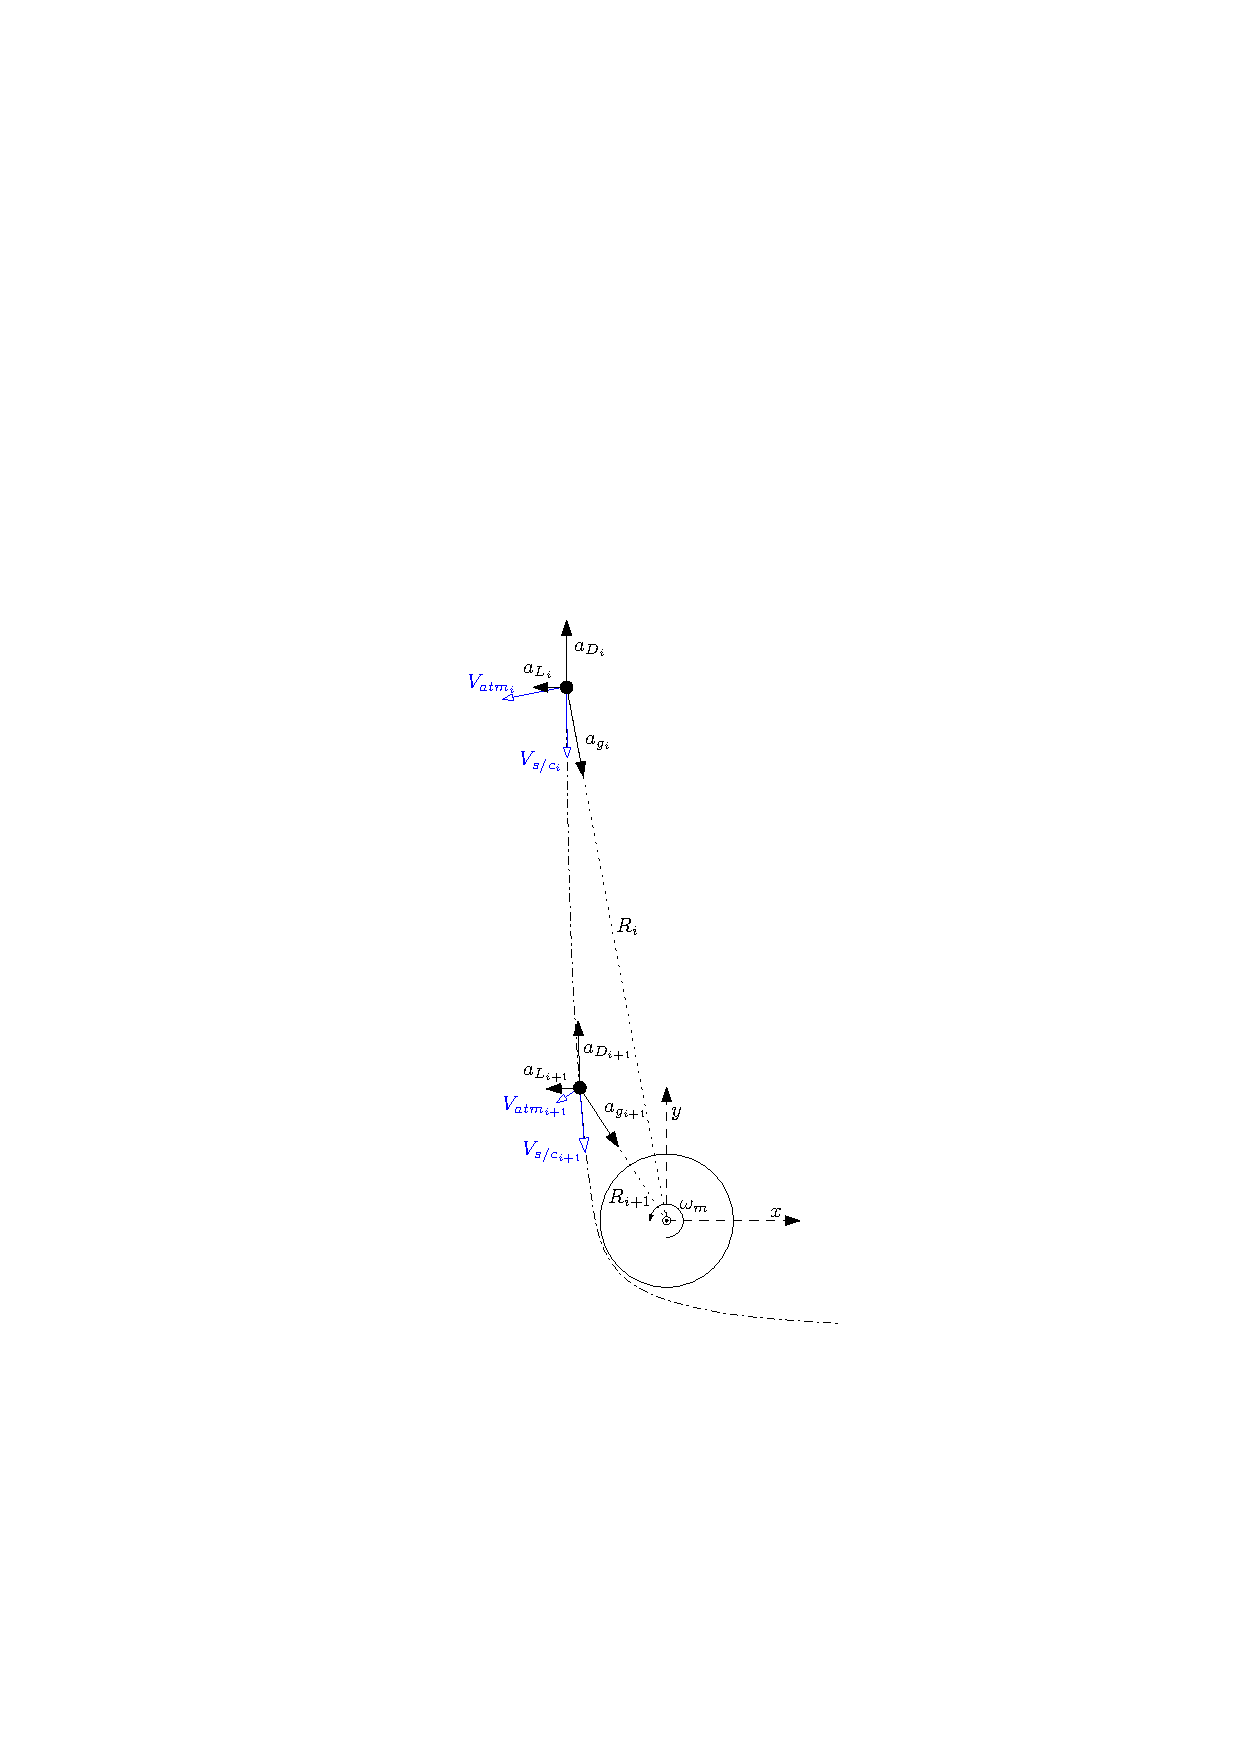
\includegraphics[width = 0.4\textwidth]{Figure/orbital_mechanics.pdf}
		\caption{The \gls{fbs} of the aeroshell mission}
		\label{fig:orb}
\end{wrapfigure}

The motion of a spacecraft can be broken down in some dominant contributors. These contributors are the gravitational pull and the aerodynamic forces. Disturbances like solar radiation or gravitational pull from moons or other bodies is neglected in the model.

The gravitational pull is described by Newtons law of gravitation



\subsection{Program structure}

\subsection{Verification and validation}